%============================================================================
%  ARDL-BART : A Professional Lecture
%  Non-parametric ARDL modelling with Bayesian Additive Regression Trees
%  Based on Mahdavi, Ehsani, Ahelegbey & Mohammadpour (2024),
%  Applied Mathematics 15, 292-312, doi:10.4236/am.2024.154018
%  Companion Python package:  pip install bartardl
%
%  Compile with:  pdflatex ardl_bart_lecture.tex   (run twice)
%============================================================================
\documentclass[11pt,aspectratio=169]{beamer}

\usepackage[T1]{fontenc}
\usepackage[utf8]{inputenc}
\usepackage{lmodern}
\usepackage{amsmath,amssymb,amsfonts}
\usepackage{bm}
\usepackage{booktabs}
\usepackage{array}
\usepackage{colortbl}
\usepackage{graphicx}
\usepackage{tikz}
\usepackage{pgfplots}
\pgfplotsset{compat=1.18}
\usetikzlibrary{arrows.meta,positioning,shapes.geometric,backgrounds}
\usepackage[most]{tcolorbox}
\usepackage{listings}
\usepackage{fontawesome5}

\graphicspath{{../figures/}}

%----------------------------------------------------------------------------
%  Colour palette (inspired by the MATLAB Parula map used in the package)
%----------------------------------------------------------------------------
\definecolor{parIndigo}{HTML}{352A87}   % deep indigo  (primary)
\definecolor{parBlue}{HTML}{0F6FC6}      % azure
\definecolor{parTeal}{HTML}{0FAEB9}      % teal (accent)
\definecolor{parGreen}{HTML}{65BE86}     % green
\definecolor{parGold}{HTML}{FFC337}      % gold (highlight)
\definecolor{parRed}{HTML}{C0392B}       % brick red (warning)
\definecolor{inkGrey}{HTML}{2B2D42}      % near-black text
\definecolor{softGrey}{HTML}{F4F5FA}     % panel background
\definecolor{lineGrey}{HTML}{D9DCE8}

%----------------------------------------------------------------------------
%  Beamer look
%----------------------------------------------------------------------------
\usetheme{default}
\setbeamertemplate{navigation symbols}{}
\setbeamercolor{normal text}{fg=inkGrey}
\setbeamercolor{structure}{fg=parIndigo}
\setbeamercolor{frametitle}{fg=white,bg=parIndigo}
\setbeamercolor{title}{fg=parIndigo}
\setbeamercolor{item}{fg=parTeal}
\setbeamercolor{block title}{fg=white,bg=parBlue}
\setbeamercolor{block body}{bg=softGrey}
\setbeamerfont{frametitle}{series=\bfseries}
\setbeamerfont{title}{series=\bfseries}
\setbeamertemplate{itemize items}[circle]

% coloured frame-title bar
\setbeamertemplate{frametitle}{%
  \nointerlineskip
  \begin{beamercolorbox}[wd=\paperwidth,ht=2.6ex,dp=1.2ex,leftskip=0.3cm]{frametitle}%
    \bfseries\insertframetitle%
  \end{beamercolorbox}%
}

% footline
\setbeamertemplate{footline}{%
  \leavevmode\hbox{%
    \begin{beamercolorbox}[wd=.4\paperwidth,ht=2.4ex,dp=1ex,leftskip=.3cm]{author in head/foot}%
      \color{parIndigo}\footnotesize ARDL-BART\hfill\end{beamercolorbox}%
    \begin{beamercolorbox}[wd=.6\paperwidth,ht=2.4ex,dp=1ex,rightskip=.3cm]{author in head/foot}%
      \color{inkGrey}\footnotesize\hfill\texttt{pip install bartardl}\quad
      \insertframenumber/\inserttotalframenumber\end{beamercolorbox}}%
}

%----------------------------------------------------------------------------
%  tcolorbox styles
%----------------------------------------------------------------------------
\newtcolorbox{thmbox}[1][Theory]{%
  enhanced,breakable,colback=softGrey,colframe=parIndigo,
  coltitle=white,fonttitle=\bfseries,title={#1},
  boxrule=0.8pt,arc=2pt,left=3mm,right=3mm,top=1.5mm,bottom=1.5mm}

\newtcolorbox{keybox}[1][Key idea]{%
  enhanced,breakable,colback=parGold!14,colframe=parGold!85!black,
  coltitle=inkGrey,fonttitle=\bfseries,title={\faLightbulb~~#1},
  boxrule=0.8pt,arc=2pt,left=3mm,right=3mm,top=1.5mm,bottom=1.5mm}

\newtcolorbox{exbox}[1][Applied example]{%
  enhanced,breakable,colback=parTeal!10,colframe=parTeal!85!black,
  coltitle=white,fonttitle=\bfseries,title={\faFlask~~#1},
  boxrule=0.8pt,arc=2pt,left=3mm,right=3mm,top=1.5mm,bottom=1.5mm}

\newtcolorbox{warnbox}[1][Caveat]{%
  enhanced,breakable,colback=parRed!8,colframe=parRed,
  coltitle=white,fonttitle=\bfseries,title={\faExclamationTriangle~~#1},
  boxrule=0.8pt,arc=2pt,left=3mm,right=3mm,top=1.5mm,bottom=1.5mm}

%----------------------------------------------------------------------------
%  Python listing style
%----------------------------------------------------------------------------
\lstdefinestyle{py}{%
  language=Python,
  basicstyle=\ttfamily\scriptsize\color{inkGrey},
  keywordstyle=\color{parIndigo}\bfseries,
  stringstyle=\color{parGreen!70!black},
  commentstyle=\color{parBlue!70!black}\itshape,
  numberstyle=\tiny\color{lineGrey!60!black},
  emph={bartardl,ba,BART,ARDLBART,Lasso,ElasticNet,BayesianNetwork,friedman,
        load_macro,rmse,relative_rmse,simulation_table,ranking_table,
        parula_colors,inclusion_plot,rmse_boxplot,journal_table},
  emphstyle=\color{parTeal!80!black}\bfseries,
  showstringspaces=false,
  columns=fullflexible,
  keepspaces=true,
  breaklines=true,
  frame=single,
  rulecolor=\color{lineGrey},
  backgroundcolor=\color{softGrey},
  framexleftmargin=2mm,
  xleftmargin=2mm,
  aboveskip=2pt,belowskip=2pt,
}
\lstset{style=py}

% section divider frames
\newcommand{\partdivider}[2]{%
\begin{frame}[plain]
  \begin{tikzpicture}[remember picture,overlay]
    \fill[parIndigo] (current page.south west) rectangle (current page.north east);
    \fill[parTeal] ([yshift=-3.2cm]current page.north west) rectangle
                   ([yshift=-3.6cm]current page.north east);
  \end{tikzpicture}
  \vspace{1.2cm}
  {\color{parGold}\Large\bfseries Part #1}\\[4mm]
  {\color{white}\Huge\bfseries #2}
\end{frame}}

\newcommand{\code}[1]{{\ttfamily\color{parIndigo}#1}}

%============================================================================
\begin{document}

%---------------------------------------------------------------- title -----
\begin{frame}[plain]
  \begin{tikzpicture}[remember picture,overlay]
    \fill[parIndigo] (current page.south west) rectangle (current page.north east);
    \begin{scope}
      \clip (current page.south west) rectangle (current page.north east);
      \foreach \i in {0,...,18}{
        \fill[parTeal,opacity=0.06] ([xshift=\i cm]current page.west) circle (3.2cm);}
    \end{scope}
    \fill[parGold] ([yshift=-4.3cm]current page.north west) rectangle
                   ([yshift=-4.45cm]current page.north east);
  \end{tikzpicture}
  \vspace{0.6cm}
  {\color{white}\Huge\bfseries Measuring Causal Effect with\\[2mm] ARDL--BART}\\[3mm]
  {\color{parGold}\large A non-parametric distributed-lag model with\\
   Bayesian Additive Regression Trees}\\[10mm]
  {\color{white}\normalsize Theory, evidence, and a hands-on \texttt{Python} tutorial}\\[8mm]
  {\color{white!85}\small Companion package: \texttt{\color{parGold}pip install bartardl}
   \quad\textbullet\quad \faGithub~ github.com/merwanroudane/bartardl}\\[2mm]
  {\color{white!70}\footnotesize After Mahdavi, Ehsani, Ahelegbey \& Mohammadpour (2024),
   \emph{Applied Mathematics} \textbf{15}, 292--312.}
\end{frame}

%---------------------------------------------------------------- outline ----
\begin{frame}{Roadmap}
  \setbeamertemplate{enumerate items}[circle]
  \begin{columns}[T]
    \begin{column}{0.5\textwidth}
      \begin{enumerate}
        \item[\textcolor{parTeal}{\faCompass}] \textbf{Motivation \& the ARDL set-up}
        \item[\textcolor{parTeal}{\faTree}] \textbf{BART theory}\\ {\small sum-of-trees, priors, MCMC}
        \item[\textcolor{parTeal}{\faProjectDiagram}] \textbf{The competitors}\\ {\small LASSO, Elastic Net, Bayesian network}
      \end{enumerate}
    \end{column}
    \begin{column}{0.5\textwidth}
      \begin{enumerate}
        \item[\textcolor{parGold}{\faChartBar}] \textbf{Simulation evidence}
        \item[\textcolor{parGold}{\faGlobe}] \textbf{Macroeconomic application}
        \item[\textcolor{parGold}{\faLaptopCode}] \textbf{Applied lab with \texttt{bartardl}}
        \item[\textcolor{parGold}{\faFlagCheckered}] \textbf{Guidance \& take-aways}
      \end{enumerate}
    \end{column}
  \end{columns}
  \vspace{4mm}
  \begin{keybox}[The one-sentence summary]
   Replace the \emph{linear} conditional mean of an ARDL equation by a
   \textbf{sum of Bayesian regression trees}, so lag effects may be non-linear
   and interactive --- then benchmark it honestly against penalised-regression selectors.
  \end{keybox}
\end{frame}

%============================================================ PART I =========
\partdivider{I}{Motivation \& the ARDL set-up}

\begin{frame}{Why go non-linear?}
  \begin{columns}[T]
    \begin{column}{0.56\textwidth}
      Traditional macro models --- VAR, dynamic factor, linear projection ---
      share one limitation:
      \begin{itemize}
        \item they impose a \textcolor{parIndigo}{\bfseries linear, additive}
              response surface;
        \item no threshold effects (e.g.\ policy rates), no interactions,
              no regime changes;
        \item misspecification $\Rightarrow$ biased forecasts and misleading
              policy read-offs.
      \end{itemize}
      \vspace{2mm}
      Macro relationships are widely believed to be \textbf{non-linear}.
      We want a model that \emph{learns} the shape of $f$ from data.
    \end{column}
    \begin{column}{0.44\textwidth}
      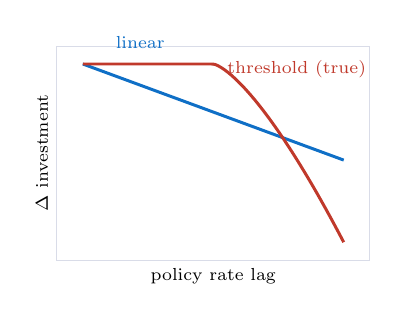
\begin{tikzpicture}[scale=0.9]
        \begin{axis}[width=6cm,height=4.6cm,
            xlabel={\scriptsize policy rate lag},ylabel={\scriptsize $\Delta$ investment},
            xtick=\empty,ytick=\empty,axis line style={lineGrey},
            tick style={draw=none},clip=false]
          \addplot[parBlue,very thick,domain=0:5,samples=50]{2-0.35*x};
          \addplot[parRed,very thick,domain=0:5,samples=80]{2-0.9*max(x-2.5,0)^1.4};
          \node[parBlue] at (axis cs:1.1,2.4){\scriptsize linear};
          \node[parRed] at (axis cs:4.1,1.9){\scriptsize threshold (true)};
        \end{axis}
      \end{tikzpicture}\\[1mm]
      {\scriptsize A linear fit misses the kink where investment collapses once
       rates cross a threshold.}
    \end{column}
  \end{columns}
\end{frame}

\begin{frame}{The ARDL equation --- ``a VAR, one equation at a time''}
  \begin{thmbox}[Single-equation ARDL]
   For a target $y$ and a system of $K$ variables $x_1,\dots,x_K$,
   \[
     y_t \;=\; f\!\big(y_{t-1},\dots,y_{t-p},\,x_{1,t-1},\dots,x_{K,t-p}\big)\;+\;e_t,
     \qquad e_t\sim N(0,\sigma^2).
   \]
   Every variable enters at lags $1,\dots,p$; equations are estimated
   \textbf{one at a time} (no cross-equation error covariance).
  \end{thmbox}
  \vspace{1mm}
  \begin{columns}[T]
    \begin{column}{0.5\textwidth}
      \textbf{Classical ARDL:} $f$ is \emph{linear} $\Rightarrow$ OLS.\\[1mm]
      \textbf{This lecture:} $f$ is \emph{unknown} and estimated
      \textcolor{parTeal}{\bfseries non-parametrically with BART}.
    \end{column}
    \begin{column}{0.5\textwidth}
      \begin{warnbox}[Naming, kept honest]
        Here ``ARDL'' means the distributed-lag \emph{regression} (no bounds
        test / no error-correction term), and ``causal effect'' is operationalised
        as \emph{forecasting + variable importance} --- exactly what the paper does.
      \end{warnbox}
    \end{column}
  \end{columns}
\end{frame}

%============================================================ PART II ========
\partdivider{II}{BART theory}

\begin{frame}{The sum-of-trees model}
  \begin{thmbox}[Bayesian Additive Regression Trees (Chipman, George \& McCulloch, 2010)]
   \[
     y=f(\bm x)+\varepsilon,\quad \varepsilon\sim N(0,\sigma^2),
     \qquad
     f(\bm x)\;\approx\;\sum_{l=1}^{m} g(\bm x;\,T_l,\,M_l).
   \]
   Each $T_l$ is a binary \emph{decision tree} (split rules); $M_l=\{\mu_{l1},\dots\}$
   are its \emph{leaf parameters}. The ensemble is a sum of $m$ \textbf{weak learners}.
  \end{thmbox}
  \begin{columns}[T]
    \begin{column}{0.52\textwidth}
      \begin{keybox}[Boosting, but Bayesian]
        Like boosting, BART adds many shallow trees; \emph{unlike} boosting, a
        \textbf{prior} keeps each tree small and a \textbf{posterior} quantifies
        uncertainty in $f$ and $\sigma$.
      \end{keybox}
    \end{column}
    \begin{column}{0.48\textwidth}
      \centering
      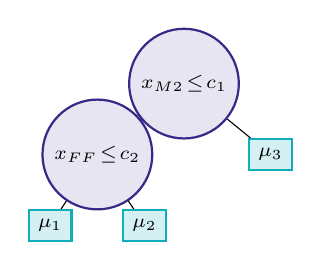
\begin{tikzpicture}[every node/.style={font=\scriptsize},level distance=9mm,
          level 1/.style={sibling distance=22mm},
          level 2/.style={sibling distance=12mm}]
        \node[circle,draw=parIndigo,fill=parIndigo!12,thick]{$x_{M2}\!\le\! c_1$}
          child{node[circle,draw=parIndigo,fill=parIndigo!12,thick]{$x_{FF}\!\le\! c_2$}
            child{node[draw=parTeal,fill=parTeal!18,thick]{$\mu_1$}}
            child{node[draw=parTeal,fill=parTeal!18,thick]{$\mu_2$}}}
          child{node[draw=parTeal,fill=parTeal!18,thick]{$\mu_3$}};
      \end{tikzpicture}\\[1mm]
      {\scriptsize one tree $g(\bm x;T_l,M_l)$: follow the rules to a leaf value $\mu$.}
    \end{column}
  \end{columns}
\end{frame}

\begin{frame}{Three priors that do the regularising}
  \begin{columns}[T]
    \begin{column}{0.34\textwidth}
      \begin{thmbox}[1. Tree structure]
        A node at depth $d$ splits with probability
        \[\alpha\,(1+d)^{-\beta}.\]
        Defaults $\alpha=0.95,\ \beta=2$ make deep trees very unlikely
        $\Rightarrow$ shallow, weak trees.
      \end{thmbox}
    \end{column}
    \begin{column}{0.32\textwidth}
      \begin{thmbox}[2. Leaf value]
        With $y$ scaled to $[-\tfrac12,\tfrac12]$,
        \[\mu\sim N(0,\tau),\quad \tau=\Big(\tfrac{0.5}{k\sqrt m}\Big)^{\!2}.\]
        $k{=}2$: the $m$ leaves sum to cover the data range in $\pm k$ SDs.
      \end{thmbox}
    \end{column}
    \begin{column}{0.34\textwidth}
      \begin{thmbox}[3. Error variance]
        \[\sigma^2\sim \text{InvGamma}(\tfrac{\nu}{2},\tfrac{\nu\lambda}{2}),\]
        $\lambda$ set so $\Pr(\sigma<\hat\sigma)=q$ from an OLS pilot.
        Defaults $\nu{=}3,\ q{=}0.9$.
      \end{thmbox}
    \end{column}
  \end{columns}
  \vspace{2mm}
  \begin{keybox}[Regularisation prior]
    No single tree may explain much: the depth prior shrinks trees, the leaf
    prior shrinks $\mu$ toward $0$. Signal is built up \emph{additively} across
    the ensemble --- this is why BART resists over-fitting.
  \end{keybox}
\end{frame}

\begin{frame}{Posterior sampling: Bayesian back-fitting MCMC}
  \begin{thmbox}[Gibbs sweep]
   For each tree $j=1,\dots,m$ compute the \emph{partial residual}
   \[
     R_j \;=\; y-\sum_{h\neq j} g(\bm x;T_h,M_h),
   \]
   update $(T_j,M_j)$ given $R_j$, then draw $\sigma^2$ from its full conditional.
  \end{thmbox}
  \begin{enumerate}\small
    \item \textbf{Structure move} on $T_j$: a Metropolis--Hastings \emph{grow} or
          \emph{prune} proposal (accept/reject).
    \item \textbf{Leaf draw}: each $\mu$ from its conjugate normal posterior
          $\;\mu\mid R_j\sim N\!\big(\text{mean},\,1/\text{prec}\big)$,
          $\;\text{prec}=1/\tau+n_{\text{leaf}}/\sigma^2$.
    \item \textbf{Noise draw}: $\sigma^2\sim\text{InvGamma}\!\big(\tfrac{\nu+n}{2},\,
          \tfrac{\nu\lambda+\sum e^2}{2}\big)$.
  \end{enumerate}
  \begin{keybox}[Efficiency]
    Keep a running total fit and each tree's contribution: the partial residual
    is an $O(n)$ update, not a full re-evaluation of the ensemble.
  \end{keybox}
\end{frame}

\begin{frame}{The grow / prune acceptance ratio}
  Choosing split variable and value \emph{uniformly} makes the rule probability
  cancel, leaving a compact log-acceptance for a \textbf{grow} at depth $d$:
  \begin{thmbox}[Log acceptance (grow); $b$ leaves before, $w_2$ nog-nodes after]
   \[
     \log A=\underbrace{\log p_d+2\log(1{-}p_{d+1})-\log(1{-}p_d)}_{\text{tree prior}}
     +\underbrace{\log\tfrac{1-p_g}{p_g}+\log\tfrac{b}{w_2}}_{\text{transition}}
     +\underbrace{\mathrm{LL}_L+\mathrm{LL}_R-\mathrm{LL}_P}_{\text{marginal likelihood}}
   \]
   with $p_d=\alpha(1+d)^{-\beta}$ and, for a node of $n$ residuals summing to $s$,
   \[
     \mathrm{LL}(n,s)=\tfrac12\log\!\frac{\sigma^2}{\sigma^2+n\tau}
     +\frac{\tau\,s^2}{2\sigma^2(\sigma^2+n\tau)} .
   \]
  \end{thmbox}
  \textbf{Prune} is the exact reverse move. The leaf value $\mu$ is integrated out
  in $\mathrm{LL}$, which is what makes the trees mix well.
\end{frame}

\begin{frame}{Variable importance: inclusion proportions}
  \begin{columns}[T]
    \begin{column}{0.55\textwidth}
      \begin{thmbox}[Inclusion proportion]
        The share of \emph{all} splitting rules, across post-burn-in draws and
        all $m$ trees, that use predictor $x_j$:
        \[
          \widehat{\text{IP}}_j=\frac{\#\{\text{splits on }x_j\}}{\#\{\text{splits}\}} ,
          \qquad \sum_j \widehat{\text{IP}}_j = 1 .
        \]
      \end{thmbox}
      A large $\widehat{\text{IP}}_j$ $\Rightarrow$ $x_j$ is repeatedly useful for
      partitioning the response $\Rightarrow$ an ``important'' driver.
      \\[2mm]
      In package terms: \code{model.inclusion\_proportion\_}.
    \end{column}
    \begin{column}{0.45\textwidth}
      \begin{keybox}[Reading it well]
        With \emph{many} noise predictors, BART concentrates its splits on the
        few relevant ones --- detecting low-dimensional structure in a
        high-dimensional lag matrix (here $8\times4=32$ regressors).
      \end{keybox}
    \end{column}
  \end{columns}
\end{frame}

%============================================================ PART III =======
\partdivider{III}{The competitors}

\begin{frame}{Three ``black-box'' benchmarks}
  \begin{columns}[T]
    \begin{column}{0.33\textwidth}
      \begin{thmbox}[LASSO]
        \[\min_\beta \tfrac12\|y-X\beta\|^2+\lambda\|\beta\|_1\]
        L1 penalty $\Rightarrow$ sparse selection. CV picks $\lambda$.
      \end{thmbox}
    \end{column}
    \begin{column}{0.33\textwidth}
      \begin{thmbox}[Elastic Net]
        \[+\ \lambda\big(\alpha\|\beta\|_1+\tfrac{1-\alpha}{2}\|\beta\|_2^2\big)\]
        Handles correlated groups; $\alpha{=}1$ is LASSO, $\alpha{=}0$ is ridge.
      \end{thmbox}
    \end{column}
    \begin{column}{0.33\textwidth}
      \begin{thmbox}[Bayesian network]
        Spike-and-slab / SSVS: $\gamma_j{=}1$ is a present \emph{edge}
        $x_j\!\to\!y$. Posterior $\mathbb E[\gamma_j]$ = inclusion probability.
      \end{thmbox}
    \end{column}
  \end{columns}
  \vspace{2mm}
  \begin{exbox}[The SSVS sampler, in words]
    Draw each $\beta_j$ from its normal full conditional; flip $\gamma_j$ from a
    Bernoulli comparing slab vs.\ spike density at the current $\beta_j$; draw
    $\sigma^2$. Edges present most often are the ``network'' of drivers.
  \end{exbox}
  \begin{keybox}[Why these three]
    All are \emph{black-box predictors} like BART, so the comparison is fair:
    who best forecasts and best identifies the relevant lags?
  \end{keybox}
\end{frame}

%============================================================ PART IV ========
\partdivider{IV}{Simulation evidence}

\begin{frame}{Design: the Friedman (1991) data-generating processes}
  \begin{columns}[T]
    \begin{column}{0.55\textwidth}
      $\bm x\sim \text{Uniform}(0,1)^p$; only $x_1,\dots,x_5$ matter, the rest are noise.
      \begin{thmbox}[Non-linear DGP]
        \[y=10\sin(\pi x_1 x_2)+20(x_3-\tfrac12)^2+10x_4+5x_5+\varepsilon\]
      \end{thmbox}
      \begin{thmbox}[Linear DGP]
        \[y=2+3(x_1+x_2+x_3+x_4+x_5)+\varepsilon\]
      \end{thmbox}
      $p\in\{10,100\}$; metric = \emph{relative} RMSE (RMSE\,$/\,\sigma$; $1.0$ is perfect).
    \end{column}
    \begin{column}{0.45\textwidth}
      \begin{keybox}[The hypothesis]
        BART should \textbf{win when $f$ is non-linear} and be merely
        \emph{competitive} when $f$ is truly linear (where a linear penalty is
        unbeatable).
      \end{keybox}
    \end{column}
  \end{columns}
\end{frame}

\begin{frame}{Result 1 --- non-linear DGP: BART wins}
  \begin{columns}[T]
    \begin{column}{0.52\textwidth}
      \centering
      {\footnotesize\textbf{Relative RMSE}, $p=10$}\\[1mm]
      \begin{tabular}{lcccc}
        \toprule
        \rowcolor{parIndigo!12}
        method & mean & median & Q.50 & Q.75\\
        \midrule
        \rowcolor{parGold!25}
        \textbf{BART} & \textbf{2.554} & \textbf{2.534} & 2.534 & 2.735\\
        LASSO & 2.750 & 2.741 & 2.741 & 2.951\\
        Elastic-Net & 2.753 & 2.743 & 2.743 & 2.951\\
        Bayesian-Net & 2.727 & 2.714 & 2.714 & 2.939\\
        \bottomrule
      \end{tabular}\\[2mm]
      {\scriptsize BART attains the lowest error at every quantile.}
    \end{column}
    \begin{column}{0.48\textwidth}
      \centering
      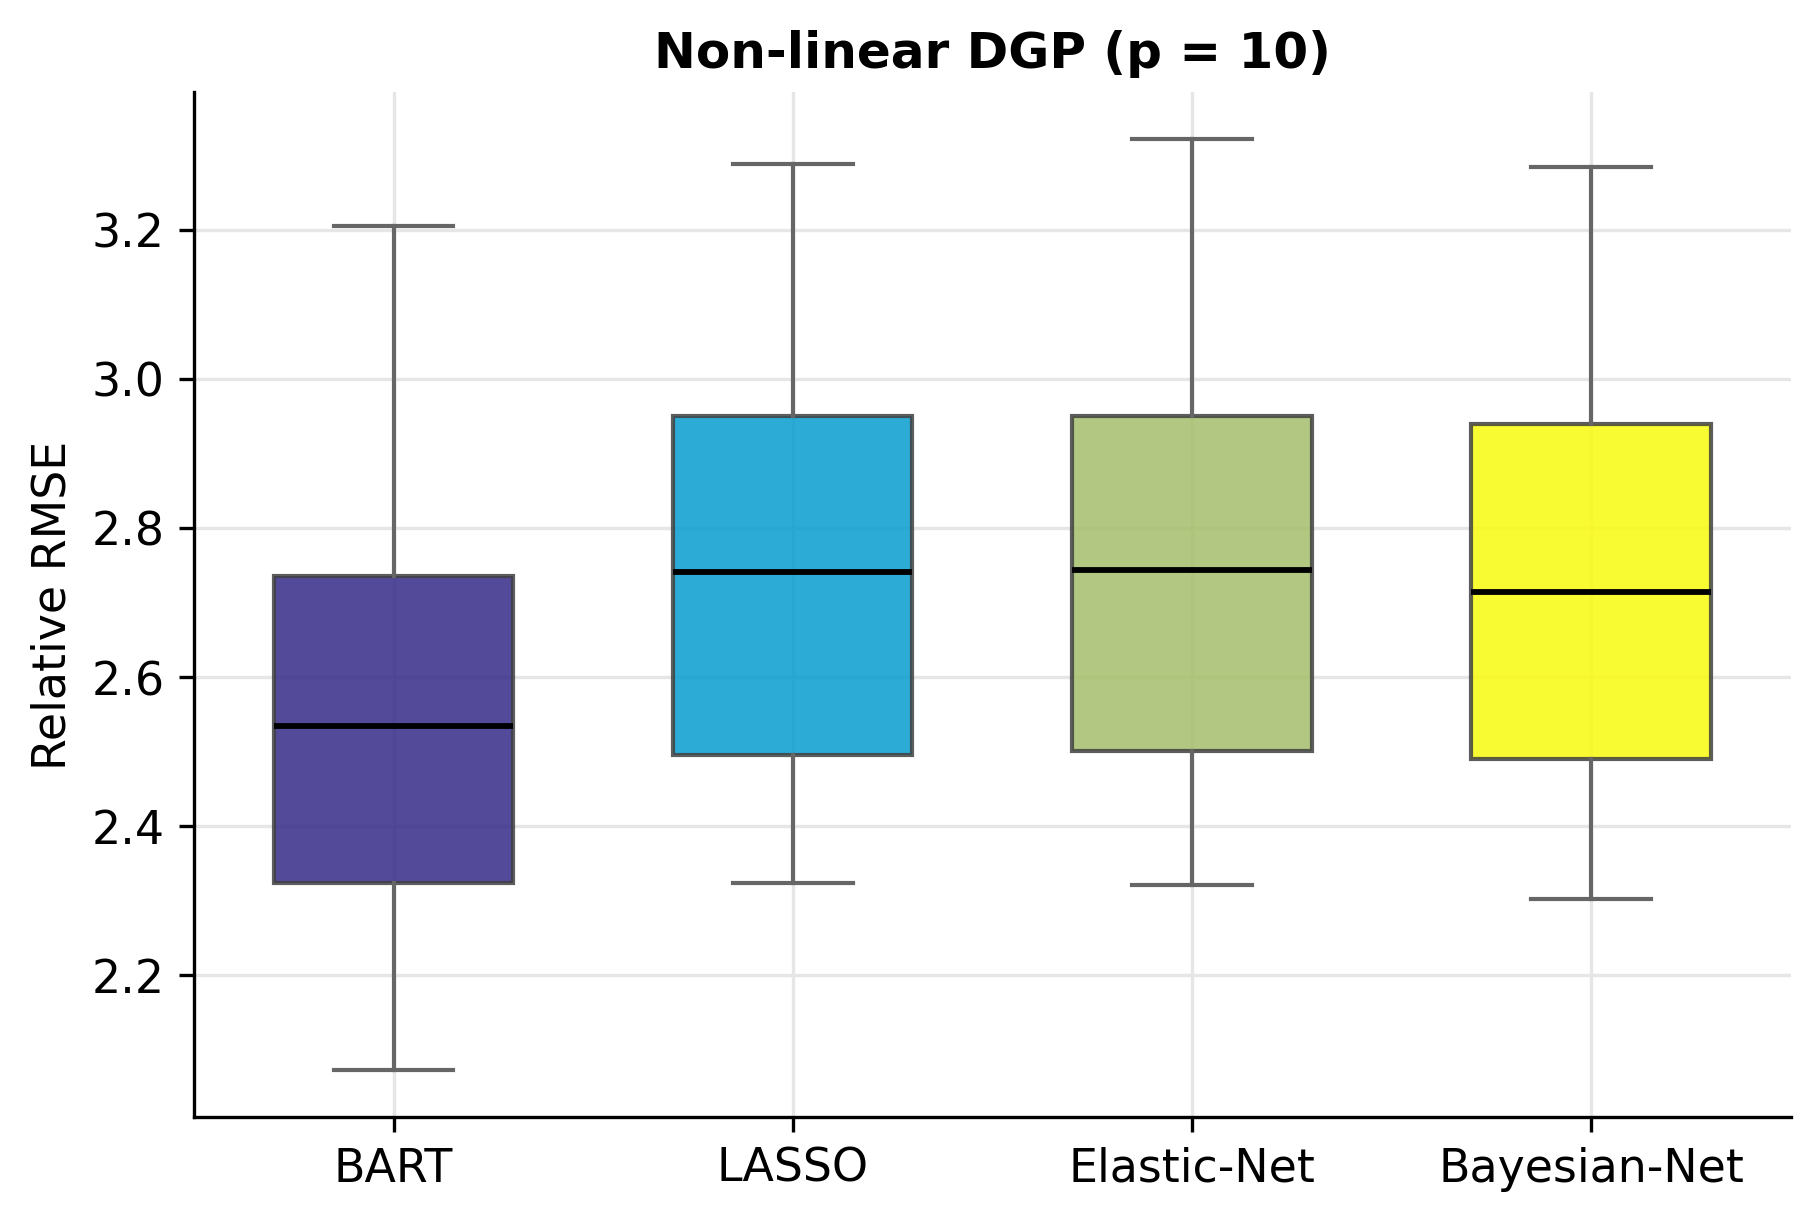
\includegraphics[width=\linewidth]{sim_nonlinear_box.png}
    \end{column}
  \end{columns}
\end{frame}

\begin{frame}{Result 1 --- and it finds the right variables}
  \begin{columns}[T]
    \begin{column}{0.5\textwidth}
      \centering
      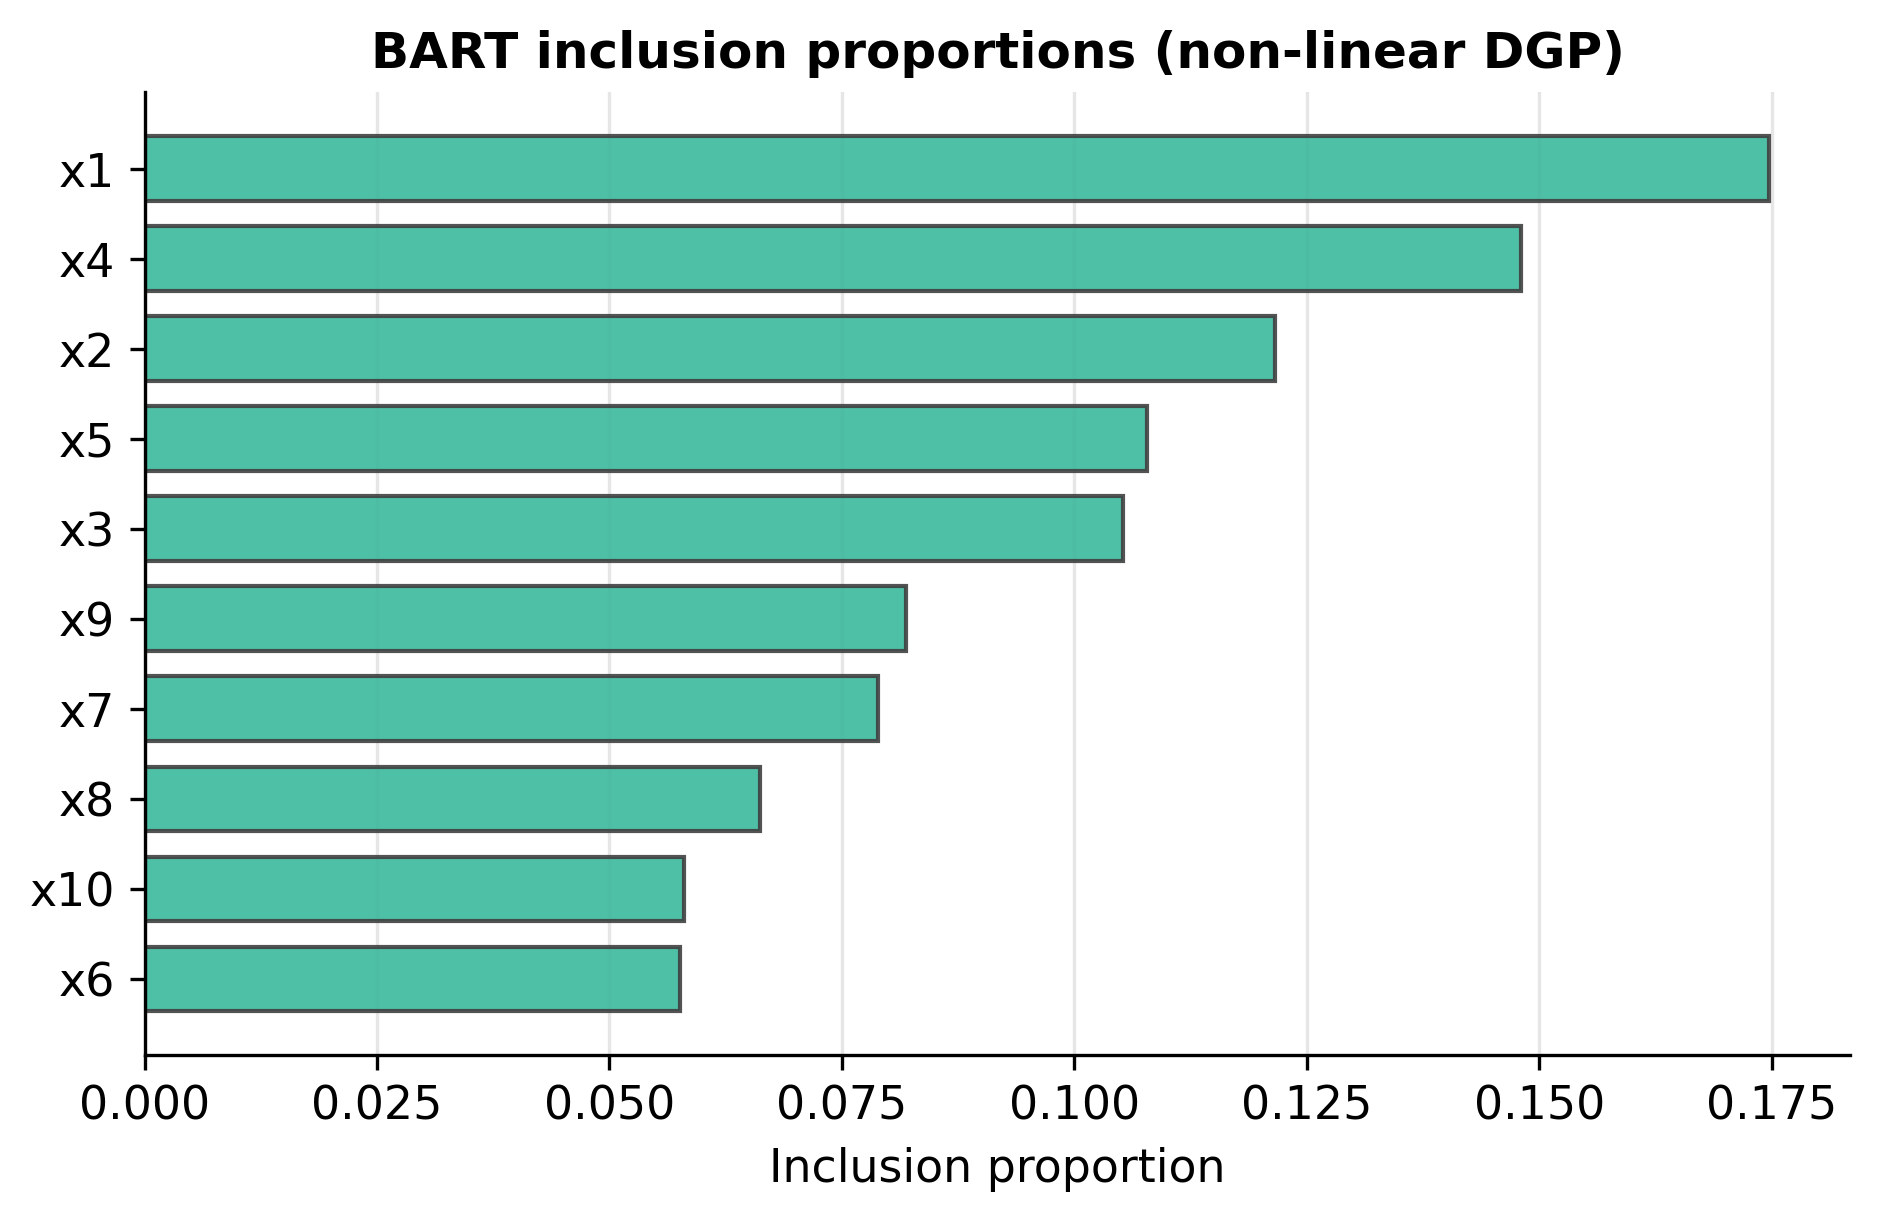
\includegraphics[width=\linewidth]{sim_nonlinear_imp.png}
    \end{column}
    \begin{column}{0.5\textwidth}
      \begin{keybox}[Low-dimensional structure]
        Inclusion proportions pile up on $x_1,\dots,x_5$; the noise predictors
        $x_6,\dots,x_{10}$ get almost no splits.
      \end{keybox}
      \begin{exbox}[Reproduce it]
        \code{python examples/02\_simulation\_nonlinear.py}
      \end{exbox}
    \end{column}
  \end{columns}
\end{frame}

\begin{frame}{Result 2 --- linear DGP: the linear selectors win}
  \begin{columns}[T]
    \begin{column}{0.52\textwidth}
      \centering
      {\footnotesize\textbf{Relative RMSE}, $p=10$}\\[1mm]
      \begin{tabular}{lcccc}
        \toprule
        \rowcolor{parIndigo!12}
        method & mean & median & Q.50 & Q.75\\
        \midrule
        BART & 1.474 & 1.418 & 1.418 & 1.530\\
        LASSO & 1.033 & 1.023 & 1.023 & 1.080\\
        Elastic-Net & 1.033 & 1.023 & 1.023 & 1.080\\
        \rowcolor{parGold!25}
        \textbf{Bayesian-Net} & \textbf{1.023} & \textbf{1.009} & 1.009 & 1.072\\
        \bottomrule
      \end{tabular}\\[2mm]
      {\scriptsize BART is competitive but not best --- exactly as expected.}
    \end{column}
    \begin{column}{0.48\textwidth}
      \centering
      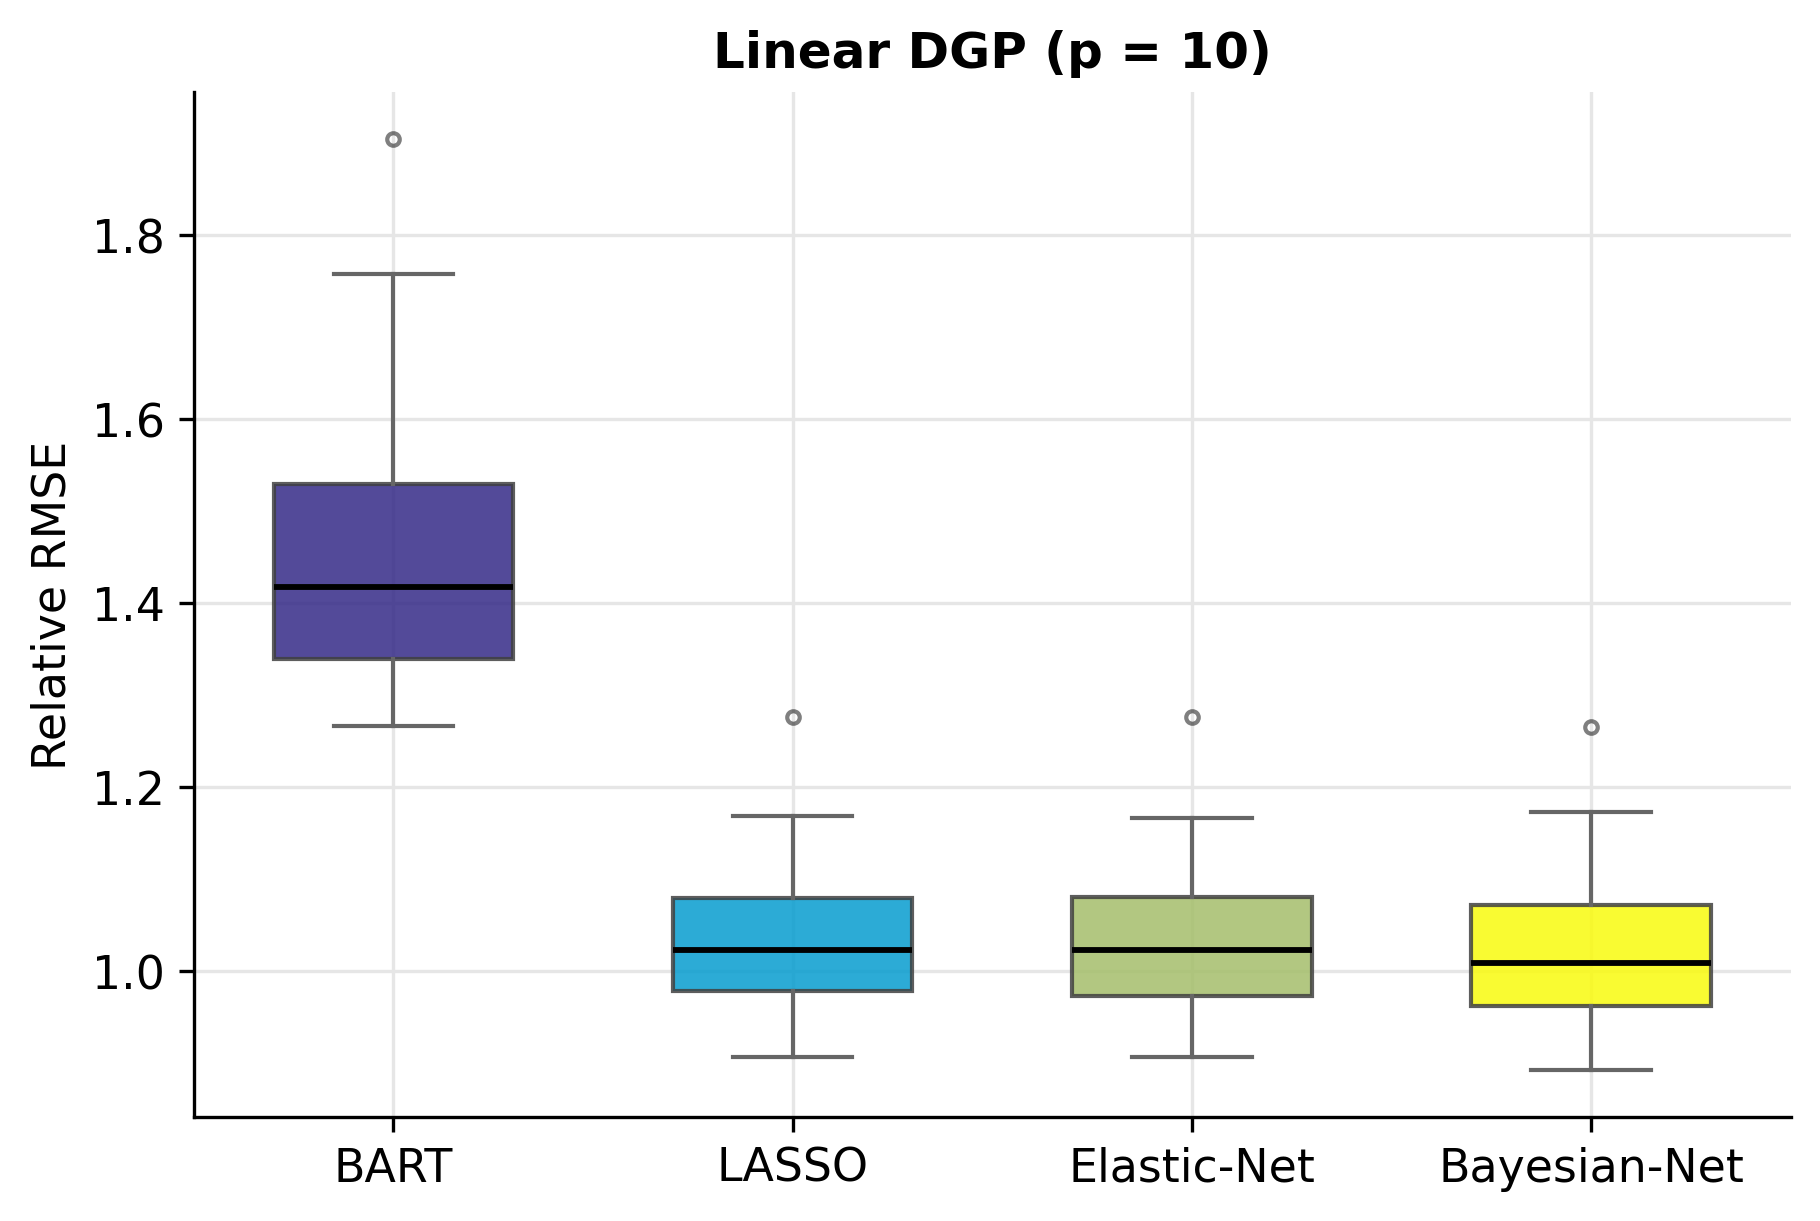
\includegraphics[width=\linewidth]{sim_linear_box.png}
    \end{column}
  \end{columns}
  \begin{keybox}[Honest science]
    A method that claimed to win \emph{everywhere} would be suspicious. BART's
    edge is specifically \textbf{non-linearity}.
  \end{keybox}
\end{frame}

%============================================================ PART V =========
\partdivider{V}{Macroeconomic application}

\begin{frame}{Data: eight US series, quarterly 1959--2022}
  \centering
  {\footnotesize Paper Table 3 --- variables and stationarity transforms}\\[1mm]
  \begin{tabular}{llcl}
    \toprule
    \rowcolor{parIndigo!12}
    ID & FRED & code & description\\
    \midrule
    GDP & GDPC1 & 5 & real gross domestic product\\
    INF & CPIAUCSL & 5 & consumer price index\\
    FF & FEDFUNDS & 2 & federal funds rate\\
    M2 & M2SL & 5 & money stock M2\\
    PC & PCECC96 & 5 & real personal consumption\\
    IP & INDPRO & 5 & industrial production\\
    U & UNRATE & 2 & unemployment rate\\
    INV & GPDIC1 & 5 & real private investment\\
    \bottomrule
  \end{tabular}\\[2mm]
  {\scriptsize code 2 $=$ first difference,\; 5 $=$ first difference of log.\quad
   ARDL(4) $\Rightarrow 8\times4=32$ regressors per equation.}
\end{frame}

\begin{frame}{Result 3 --- forecast RMSE by target (Table 4)}
  \centering
  \begin{tabular}{lcccc}
    \toprule
    \rowcolor{parIndigo!12}
    target & \textbf{BART} & LASSO & Elastic-Net & Bayesian-Net\\
    \midrule
    \rowcolor{parGold!22} GDP & \textbf{0.0032} & 0.0057 & 0.0057 & 0.0103\\
    \rowcolor{parGold!22} INF & \textbf{0.0036} & 0.0037 & 0.0037 & 0.0075\\
    FF  & 0.1216 & \textbf{0.0895} & 0.0905 & 0.0937\\
    M2  & 0.0035 & \textbf{0.0031} & 0.0031 & 0.0076\\
    \rowcolor{parGold!22} PC  & \textbf{0.0039} & 0.0056 & 0.0056 & 0.0091\\
    \rowcolor{parGold!22} IP  & \textbf{0.0037} & 0.0065 & 0.0065 & 0.0099\\
    \rowcolor{parGold!22} U   & \textbf{0.1051} & 0.1251 & 0.1252 & 0.1367\\
    \rowcolor{parGold!22} INV & \textbf{0.0118} & 0.0149 & 0.0149 & 0.0162\\
    \bottomrule
  \end{tabular}\\[2mm]
  {\color{parIndigo}\bfseries BART ranks \#1 for 6 of 8 targets};
  the linear selectors take the two (near-)linear series (FF, M2).
\end{frame}

\begin{frame}{Result 3 --- what drives GDP?}
  \begin{columns}[T]
    \begin{column}{0.5\textwidth}
      \centering
      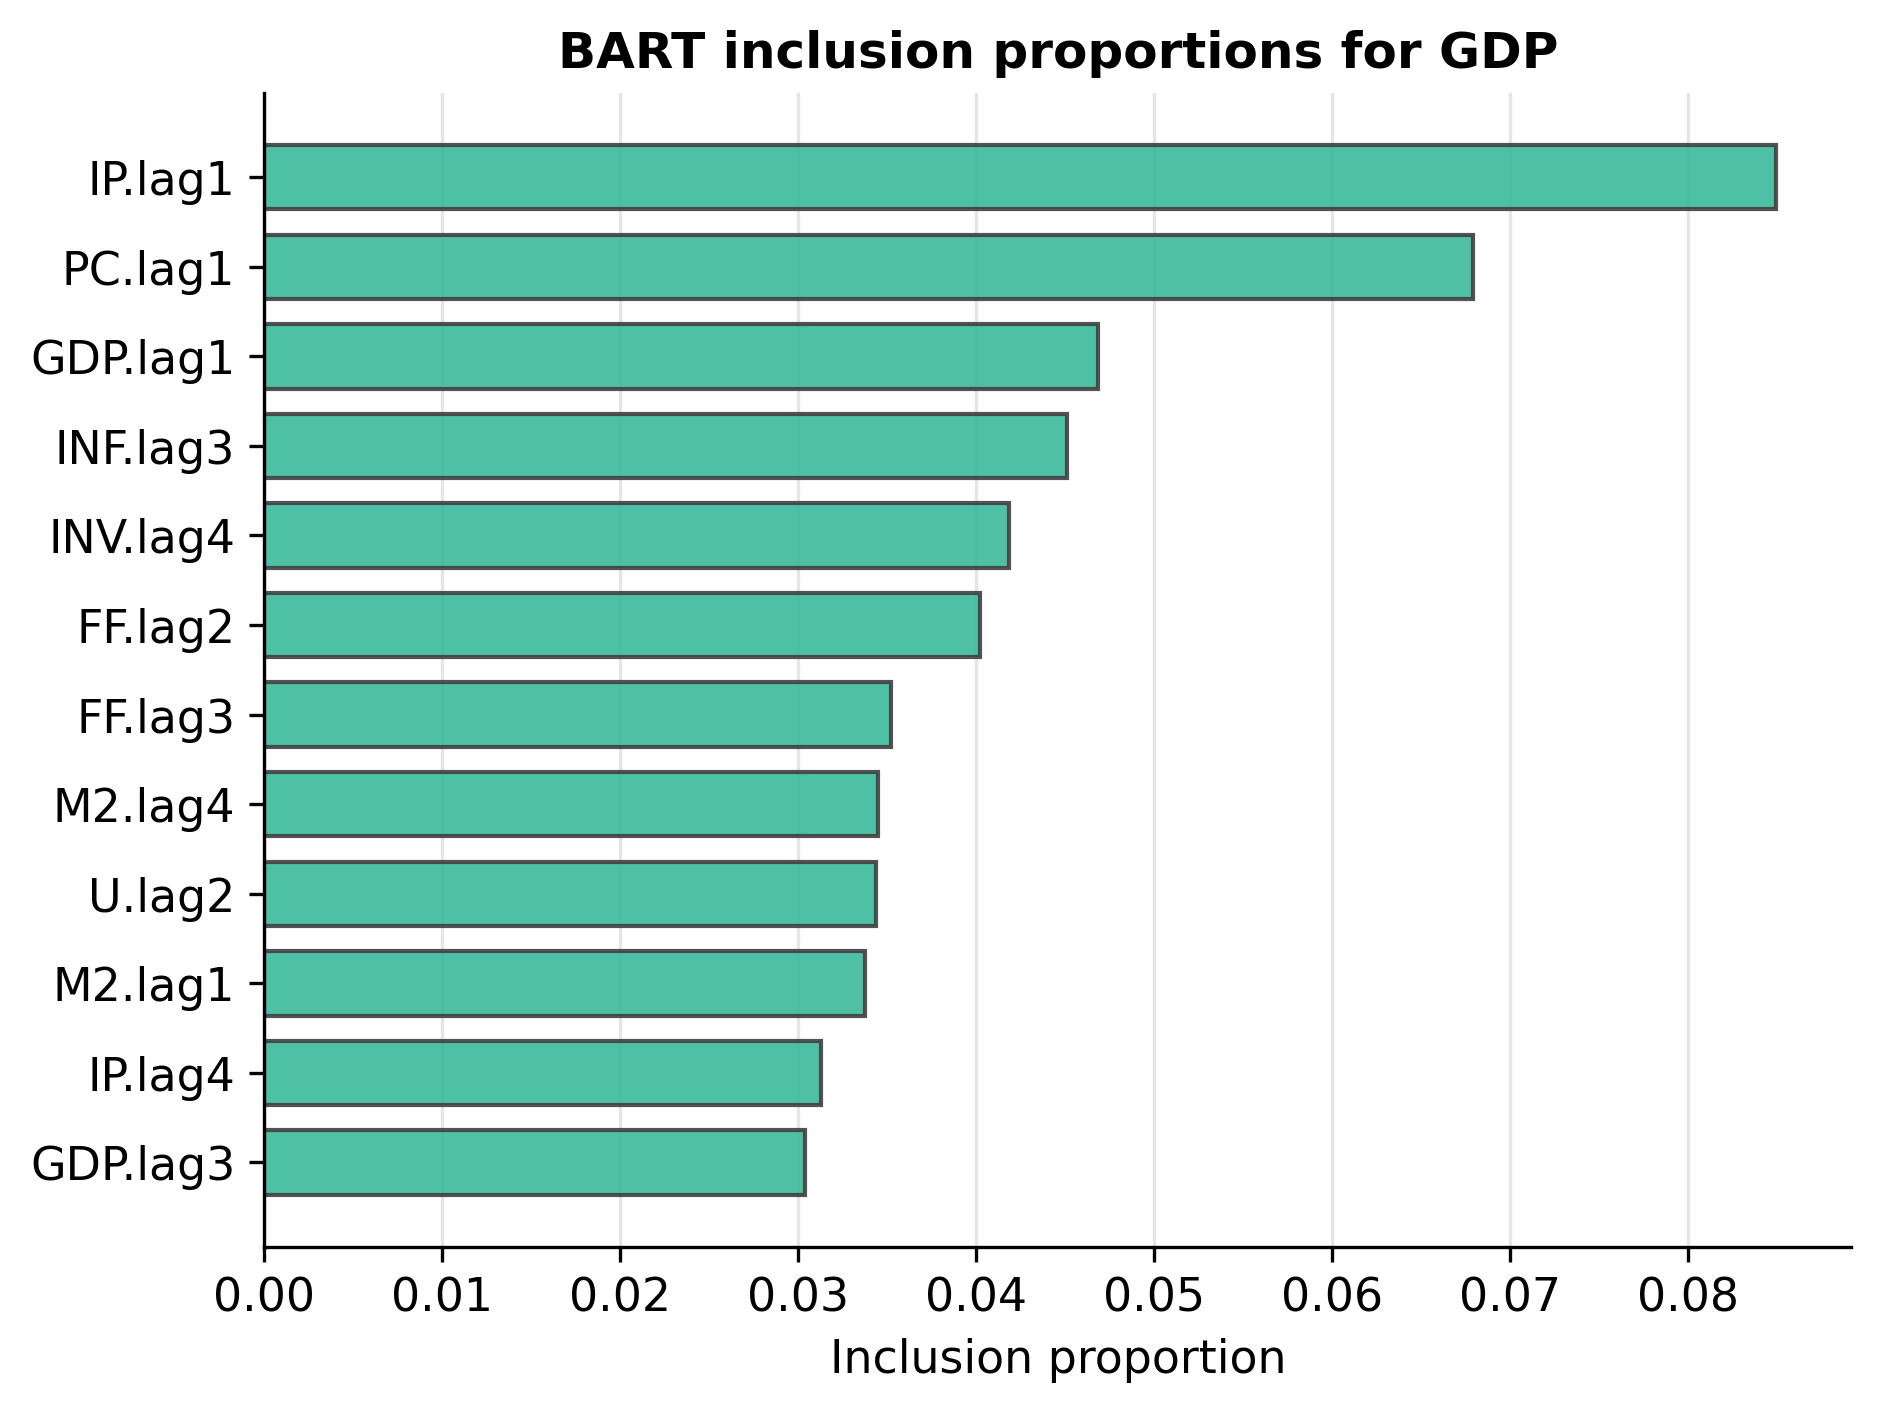
\includegraphics[width=\linewidth]{macro_gdp_imp.png}
    \end{column}
    \begin{column}{0.5\textwidth}
      \centering
      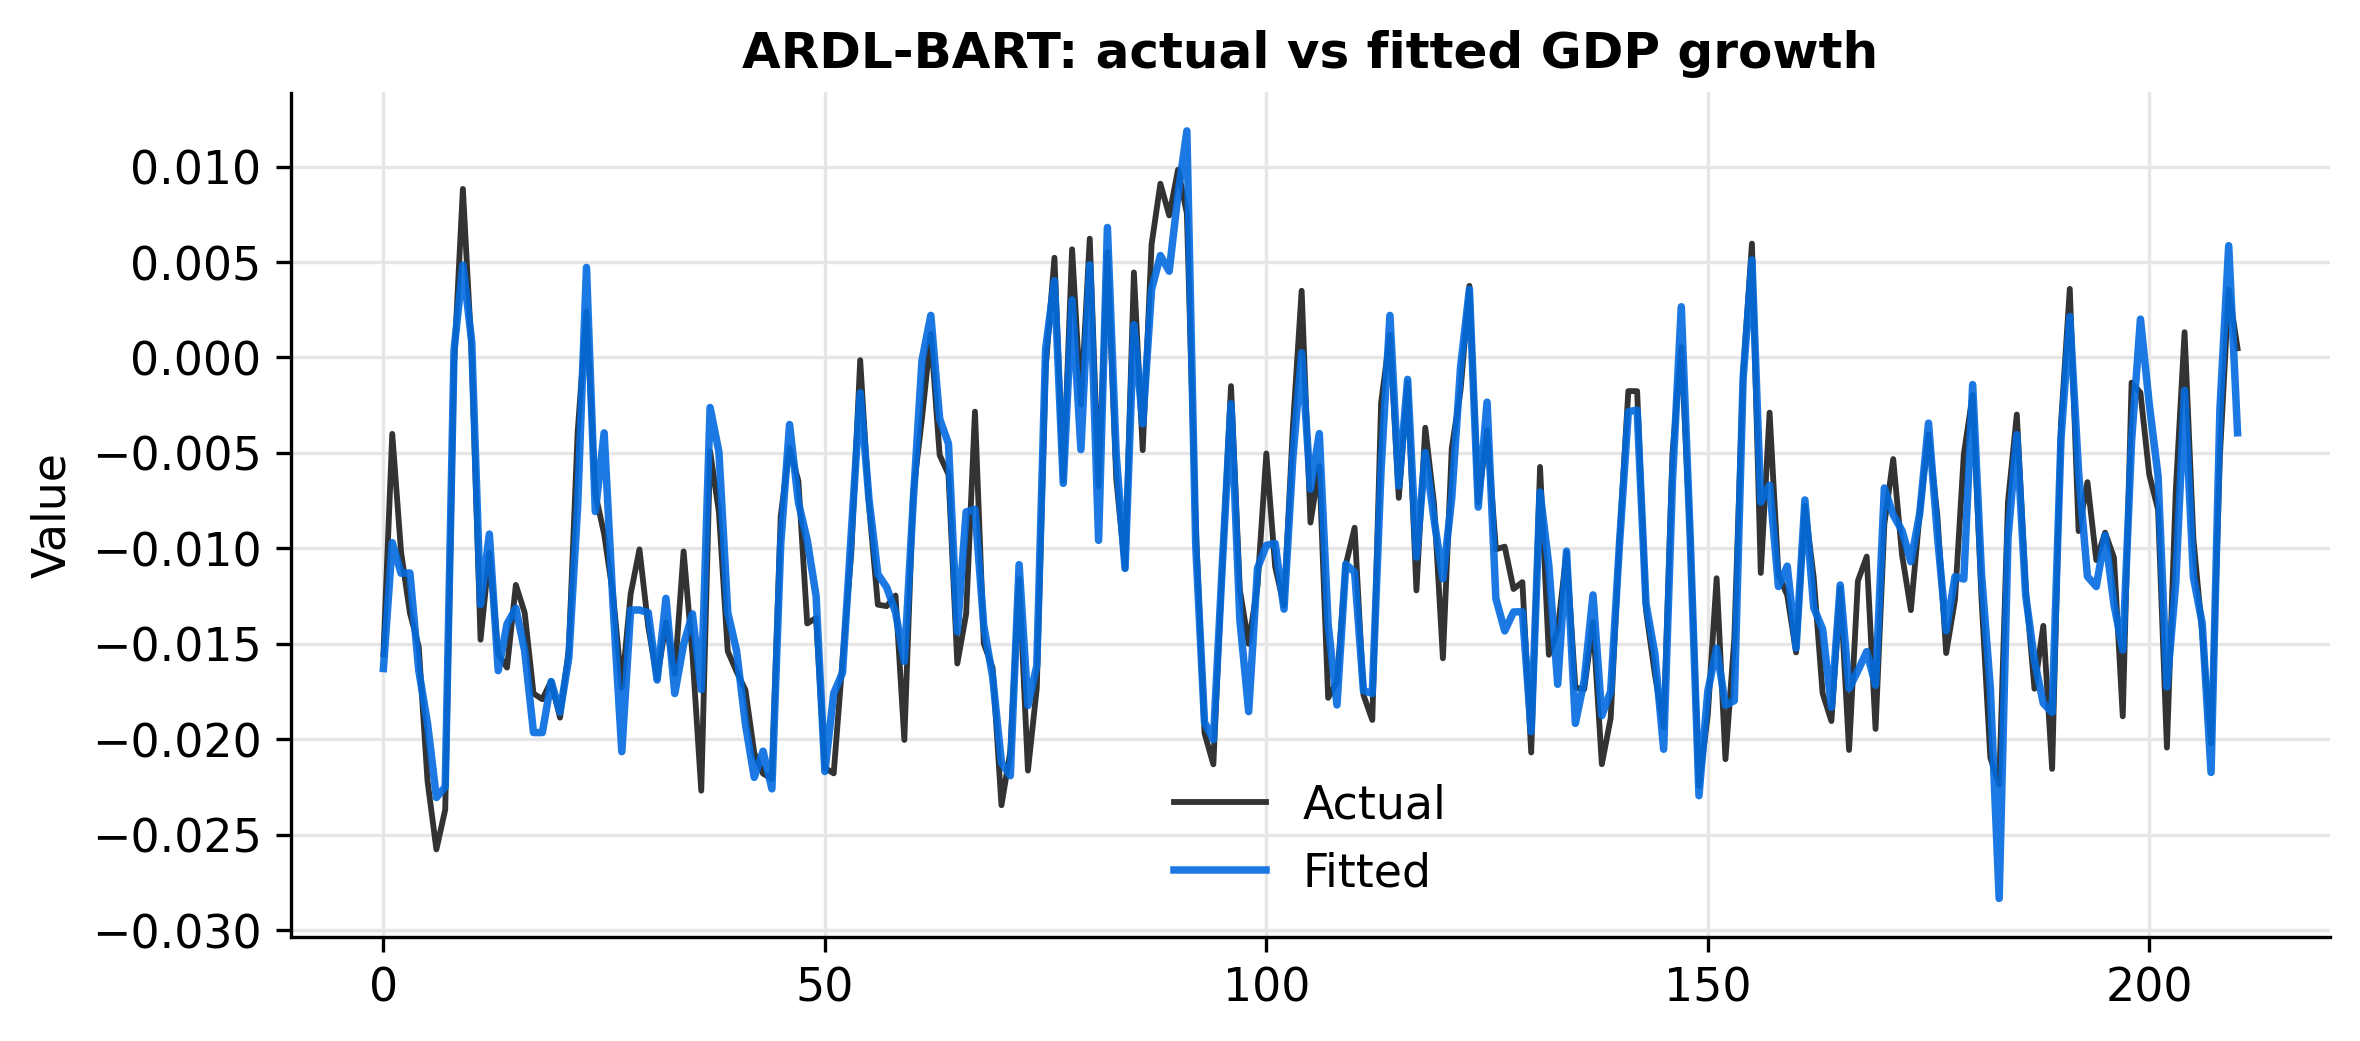
\includegraphics[width=\linewidth]{macro_gdp_fit.png}\\[1mm]
      \begin{keybox}[Interpretation]
        BART reads GDP growth off a handful of lags (consumption, industrial
        production, money, and own lags), with a close in-sample fit.
      \end{keybox}
    \end{column}
  \end{columns}
\end{frame}

%============================================================ PART VI ========
\partdivider{VI}{Applied lab with \texttt{bartardl}}

\begin{frame}[fragile]{Install \& the estimator protocol}
\begin{lstlisting}
pip install bartardl          # numpy, scipy, pandas, scikit-learn, matplotlib
\end{lstlisting}
  \begin{exbox}[One interface for every model]
    \code{BART}, \code{Lasso}, \code{ElasticNet}, \code{BayesianNetwork} all share:
  \end{exbox}
\begin{lstlisting}
est.fit(X, y)          # X: (n, p) array, y: (n,) array   -> self
est.predict(Xnew)      # -> (m,) array
est.importance_        # (p,) weights;  BART: inclusion_proportion_
\end{lstlisting}
  So any of them can be dropped into \code{ARDLBART(estimator=...)}.
\end{frame}

\begin{frame}[fragile]{Quick start --- one ARDL-BART equation}
\begin{lstlisting}
import bartardl as ba

data  = ba.load_macro()                 # stationary US macro panel (8 vars)
model = ba.ARDLBART(
    n_lags=4,
    estimator=ba.BART,
    estimator_kwargs=dict(n_trees=100, n_burn=500, n_draws=500, random_state=0),
)
res = model.fit(data, target="GDP")

print("In-sample RMSE:", ba.rmse(res.y_train, res.fitted))
print(res.top_features(5))              # 5 most influential lagged regressors
\end{lstlisting}
\begin{lstlisting}[language=,basicstyle=\ttfamily\scriptsize\color{parIndigo!85!black}]
In-sample RMSE: 0.0019
  feature variable  lag  importance
  PC.lag1       PC    1      0.0892
  IP.lag1       IP    1      0.0760
 GDP.lag1      GDP    1      0.0601
\end{lstlisting}
\end{frame}

\begin{frame}[fragile]{Simulation in five lines}
\begin{lstlisting}
draws = {"BART": [], "LASSO": []}
for rep in range(100):
    tr = ba.friedman(n=100, p=10, kind="nonlinear", random_state=rep)
    te = ba.friedman(n=100, p=10, kind="nonlinear", random_state=1000+rep)
    for name, est in [("BART", ba.BART(random_state=0)), ("LASSO", ba.Lasso())]:
        est.fit(tr.X, tr.y)
        draws[name].append(ba.relative_rmse(te.y, est.predict(te.X), 1.0))

print(ba.simulation_table(draws))       # -> Tables 1-2 layout
\end{lstlisting}
  \begin{keybox}[Match the paper exactly]
    \code{ba.BART(n\_trees=200, k=2, nu=3, q=0.9, alpha=0.95, beta=2,
    n\_draws=20000, n\_burn=250)}
  \end{keybox}
\end{frame}

\begin{frame}[fragile]{The full horse-race + ranking table}
\begin{lstlisting}
data = ba.load_macro(); H = 40; train = data.iloc[:-H]
methods = {
    "BART":         (ba.BART,            dict(n_trees=200, n_draws=1000, random_state=0)),
    "LASSO":        (ba.Lasso,           {}),
    "Elastic-Net":  (ba.ElasticNet,      {}),
    "Bayesian-Net": (ba.BayesianNetwork, dict(n_iter=2000, burn=1000, random_state=0)),
}
rmse_by_target = {}
for tgt in data.columns:
    rmse_by_target[tgt] = {}
    for name, (est, kw) in methods.items():
        m = ba.ARDLBART(n_lags=4, estimator=est, estimator_kwargs=kw).fit(train, tgt)
        pred = m.predict(data, tgt).iloc[-H:]
        rmse_by_target[tgt][name] = ba.rmse(data[tgt].loc[pred.index], pred)

print(ba.ranking_table(rmse_by_target))          # -> Table 4
\end{lstlisting}
\end{frame}

\begin{frame}[fragile]{Publication figures \& the Parula palette}
\begin{lstlisting}
from bartardl import viz
from bartardl.colors import parula_colors, get_cmap

viz.rmse_boxplot(rmse_draws, title="Non-linear DGP (p = 10)")
viz.inclusion_plot(res.importance, res.feature_names, top=12,
                   title="BART inclusion proportions for GDP")
print(viz.journal_table(rank, fmt="latex", caption="Table 4"))   # console|html|latex

parula_colors(8)          # ['#352a87', '#0268e1', ...]  MATLAB Parula stops
get_cmap("Parula")        # a Matplotlib colormap
\end{lstlisting}
  \vspace{-1mm}
  \begin{center}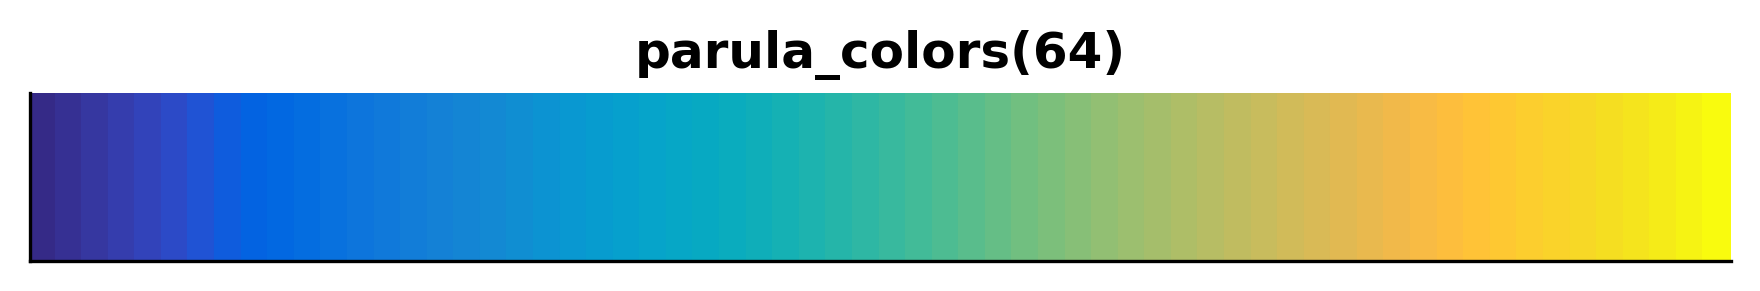
\includegraphics[width=0.78\linewidth]{parula.png}\end{center}
\end{frame}

%============================================================ PART VII =======
\partdivider{VII}{Guidance \& take-aways}

\begin{frame}{Practical guidance}
  \begin{columns}[T]
    \begin{column}{0.5\textwidth}
      \begin{keybox}[Do]
        \begin{itemize}\small
          \item Use enough trees ($m\!\approx\!200$) and draws; too few $\Rightarrow$
                noisy inclusion proportions.
          \item Stationarise first (Table 3 codes are built in).
          \item Read \emph{inclusion proportions} for importance, not $p$-values.
        \end{itemize}
      \end{keybox}
    \end{column}
    \begin{column}{0.5\textwidth}
      \begin{warnbox}[Watch out]
        \begin{itemize}\small
          \item BART \emph{extrapolates} poorly beyond the training range.
          \item Additive-tree structure can miss very strong interactions if
                under-sampled.
          \item ``Causal'' here $=$ forecasting $+$ importance, \emph{not}
                treatment effects.
        \end{itemize}
      \end{warnbox}
    \end{column}
  \end{columns}
  \vspace{1mm}
  \begin{exbox}[Uncertainty for free]
    \code{BART.yhat\_train\_draws\_} gives the full posterior of the fit
    $\Rightarrow$ 95\% bands; \code{sigma\_draws\_} gives the noise posterior.
  \end{exbox}
\end{frame}

\begin{frame}{Take-aways}
  \begin{enumerate}
    \item[\textcolor{parTeal}{\faTree}] \textbf{ARDL-BART} = single-equation
      distributed-lag regression with a \emph{non-parametric} tree-ensemble mean.
    \item[\textcolor{parTeal}{\faChartBar}] \textbf{Simulations:} BART wins under
      non-linearity, is competitive under linearity --- and recovers the relevant
      variables.
    \item[\textcolor{parGold}{\faGlobe}] \textbf{Macro data:} BART forecasts best for
      6 of 8 series, suggesting genuine non-linear dynamics.
    \item[\textcolor{parGold}{\faLaptopCode}] \textbf{Reproducible:} the entire
      pipeline is \code{pip install bartardl} --- theory, simulation, application,
      figures and tables.
  \end{enumerate}
  \vspace{3mm}
  \begin{center}
  \begin{tcolorbox}[enhanced,colback=parIndigo,colframe=parIndigo,coltext=white,
     arc=3pt,width=0.9\linewidth,halign=center]
     \large\bfseries ``Let the data choose the shape of $f$.''\\[1mm]
     \normalsize\color{parGold}\texttt{pip install bartardl}
  \end{tcolorbox}
  \end{center}
\end{frame}

\begin{frame}{References \& resources}
  \small
  \begin{itemize}
    \item Mahdavi, Ehsani, Ahelegbey \& Mohammadpour (2024).
      \emph{Measuring Causal Effect with ARDL-BART.} Applied Mathematics
      \textbf{15}, 292--312. \texttt{doi:10.4236/am.2024.154018}.
    \item Chipman, George \& McCulloch (2010). \emph{BART: Bayesian Additive
      Regression Trees.} Ann.\ Appl.\ Stat.\ \textbf{4}, 266--298.
    \item Tibshirani (1996), LASSO; Zou \& Hastie (2005), Elastic Net;
      Ahelegbey, Billio \& Casarin (2016), Bayesian graphical VAR;
      Friedman (1991), MARS.
  \end{itemize}
  \vspace{3mm}
  \begin{exbox}[Package]
    \faGithub~ \texttt{github.com/merwanroudane/bartardl} \quad\textbullet\quad
    \faBox~ \texttt{pypi.org/project/bartardl} \quad\textbullet\quad
    docs: \texttt{README.md} + \texttt{docs/guide.md}
  \end{exbox}
  \vspace{2mm}
  \centering{\color{parIndigo}\Large\bfseries Thank you \faHeart}
\end{frame}

\end{document}
